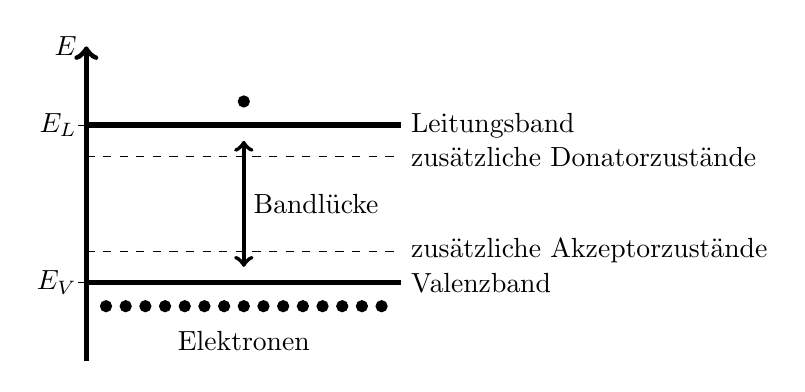
\begin{tikzpicture}
%Achse 
	\draw[draw=black,line width=2pt,->] (0,0) -- (0,4);
	\draw (-0.1,1) -- (0.1,1);
	\draw (-0.1,3) -- (0.1,3);
%Beschriftung
	\draw (0,1) node 
	  [anchor=east]
	  {$E_V$};
  \draw (0,3) node 
	  [anchor=east]
	  {$E_L$};
	\draw (0,4) node
		[anchor=east]
		{$E$};
%Bänder
	\draw[draw=black,line width=2pt] (0,1) -- (4,1);
  \draw[draw=black,line width=2pt] (0,3) -- (4,3);
	\draw (4,1) node
		[anchor=west]
		{Valenzband};
	\draw (4,3) node
		[anchor=west]
		{Leitungsband};
%Elektronen im Band
  \foreach \x in {1,2,...,15}{
	  \filldraw (\x/4,0.7) circle (2pt);}
	\filldraw (2,3.3) circle (2pt);
	\draw (2,0.5) node
		[anchor=north]
		{Elektronen};
%Bandlücke
	\draw[line width=1.5pt,<->] (2,1.2) -- (2,2.8);
	\draw (2,2) node
	  [anchor=west]
		{Bandlücke};
%Donator- und Akzeptorzustände
	\draw[dashed] (0,1.4) -- (4,1.4);
	\draw (4,1.4) node
		[anchor=west]
		{zusätzliche Akzeptorzustände};
	\draw[dashed] (0,2.6) -- (4,2.6); 
	\draw (4,2.6) node
		[anchor=west]
		{zusätzliche Donatorzustände};
\end{tikzpicture}

